Generate $n=100$ observations from $\ARMA(1,1), \AR(1)$ and $\MA(1)$ processes respectively and plot the sample ACF and PACF of each series for $\phi = 0.6, \;\theta = 0.9$. Compare the sample ACFs and PACFs of the generated series with the results given in Table 3.1. (Are these series consistent with the table?)

\notab{\center{
    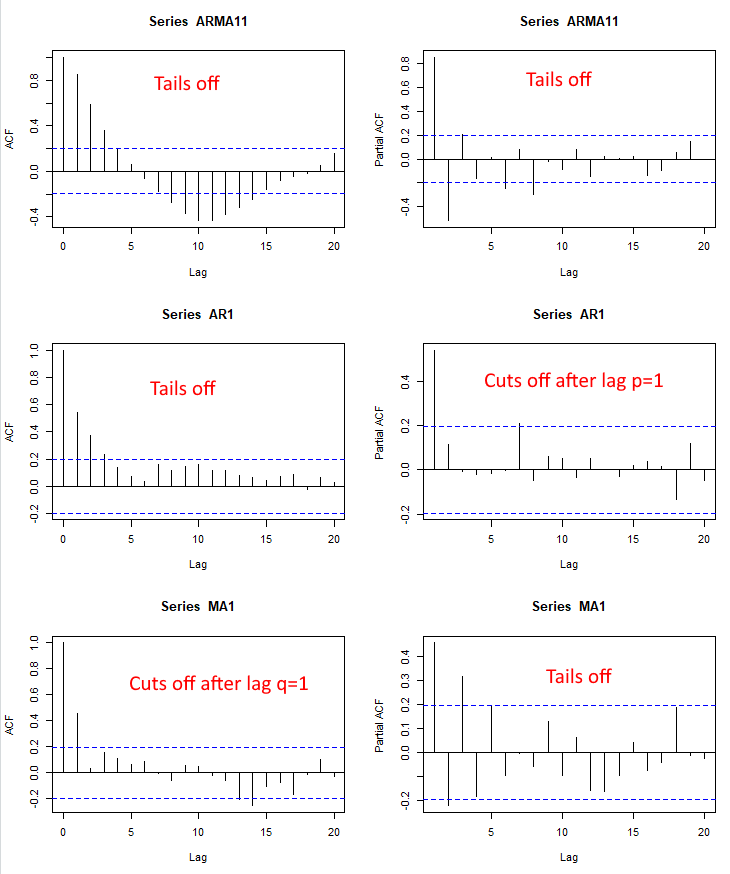
\includegraphics[width=6.25in]{img/5.PNG}
}}

From the following R code:
\begin{verbatim}
    par(mfrow = c(3,2))

    ARMA11=arima.sim(list(order=c(1,0,1), ar=.6, ma=0.9), n=100)
    acf(ARMA11)
    pacf(ARMA11)

    AR1=arima.sim(list(order=c(1,0,0), ar=.6), n=100)
    acf(AR1)
    pacf(AR1)

    MA1=arima.sim(list(order=c(0,0,1), ma=0.9), n=100)
    acf(MA1)
    pacf(MA1)
\end{verbatim}

\nl Compared to the table ({\red{red } text), these results are consistent. When the graph says it cuts off, it \textit{cuts} off. The $\AR(1)$ model looks a little misleading because R isn't labeling the start lag of 1, but tracking back from lag-5 the results hold true. Then all the ones that tail off slowly go towards zero, or oscillate around it.